\documentclass[11pt]{article}
\usepackage{graphics,graphicx}
%\usepackage[dvips]{graphics,graphicx}
\DeclareGraphicsExtensions{.ps,.jpg,.eps,.pdf,.png}
\usepackage{amsmath}
\usepackage{url}
%\usepackage{secdot}
%\usepackage{natbib}
\usepackage{verbatim, moreverb}
\bibliographystyle{plain}

%Figure path




\newcommand{\figurepath}{./figures}
\newcommand{\bibpath}{/Users/kmartin/Documents/files/misc}
\newcommand{\figfiletype}{pdf}

% Define the hangref environment used for the References list:
\newenvironment{hangref}
  {\begin{list}{}{\setlength{\itemsep}{4pt}
  \setlength{\parsep}{0pt}\setlength{\leftmargin}{+\parindent}
  \setlength{\itemindent}{-\parindent}}}{\end{list}}

% Set the page margins to 1 inch all around:
\marginparwidth 0pt\marginparsep 0pt \topskip 0pt\headsep
0pt\headheight 0pt \oddsidemargin 0pt\evensidemargin 0pt
\textwidth 6.5in \topmargin 0pt\textheight 9.0in
\newtheorem{theorem}{Theorem}


%%%%Added by Leo%%%%
\newcounter{Fig}
\renewcommand{\theFig}{\arabic{Fig}}
\newcommand{\Fig}[2]{\refstepcounter{Fig} \label{#1}
                     {\small\bf Figure \theFig.} {\small\sl #2 \par}}

\setcounter{topnumber}{3}
\renewcommand{\topfraction}{.9}
\setcounter{bottomnumber}{3}
\renewcommand{\bottomfraction}{.9}
\setcounter{totalnumber}{4}
\renewcommand{\textfraction}{.1}
\setlength{\floatsep}{.25in} 
\setlength{\intextsep}{.25in}

\setlength{\fboxrule}{2\fboxrule} \setlength{\fboxsep}{3\fboxsep}

\newcommand{\Sa}{8pt}
\newcommand{\Sb}{0pt}

\renewcommand{\_}{{\char"5F}}
\renewcommand{\{}{{\char"7B}}
\renewcommand{\}}{{\char"7D}}
\renewcommand{\^}{{\char"0D}}

\let\accute= \'
\renewcommand{\'}{{\char"0D}}

\newcommand{\bfit}{\bfseries\itshape}

\newlength{\extopskip} \newlength{\exbottomskip}
\setlength{\exbottomskip}{1\baselineskip}
\addtolength{\exbottomskip}{-5.0pt}
\setlength{\extopskip}{1\exbottomskip}
\addtolength{\extopskip}{-1\parskip}

\newenvironment{Example}{\vspace{1\extopskip}\noindent\hspace*{2em}
                         \frenchspacing\small
                         \tt\begin{tabular}{@{}l@{}}}{
                         \end{tabular}\\[1\exbottomskip]}

\newcommand{\Titem}{\item[$\triangleright$]}
\newcommand{\Ditem}{\item[$\diamond$]}

\newenvironment{Itemize}{\begin{quote}\normalsize
   \baselineskip 20pt plus .3pt minus .1pt \begin{itemize}}
   {\end{itemize}\end{quote}}
   % Set path to folder containing figures
\newcommand{\FigureFolder}{figures}
 
\begin{document}

\title{Optimization Services 1.0 User's Manual }
\vskip 2in
\author{Robert Fourer, Jun Ma, Kipp Martin}
\maketitle

\begin{abstract}
This is the User's Manual for the Optimization Services (OS) project.  The objective of  (OS) is to provide a set of standards for representing optimization instances, results, solver options, and communication between clients and solvers in a distributed environment using Web Services. This COIN-OR project provides source code for libraries and executable programs that implement OS standards. See the Optimization Services (OS) Home Site \url{www.optimizationservices.org} and the COIN-OR Trac page \url{projects.coin-or.org} for more information.
\end{abstract}


\newpage
\tableofcontents
\listoffigures
\listoftables
\hyphenation{com-plex-Type}



%\noindent\hrulefill
\newpage

\section{Introduction}

The objective of Optimization Services (OS) is to provide a set of standards for representing optimization instances, results, solver options, and communication between clients and solvers in a distributed environment using Web Services. This COIN-OR project provides source code for libraries and executable programs that implement OS standards.  See the Optimization Services (OS) Home Site \url{www.optimizationservices.org} and the COIN-OR Trac page \url{projects.coin-or.org} for more information. The OS project provides the following:

\begin{itemize}
\item[1.]  A set of XML based standards for representing optimization instances (OSiL), optimization results (OSrL), and optimization solver options (OSoL). There are other standards, but these are the main ones. The schemas for these standards are described in Section   \ref{section:schemadescriptions}.

\item[2.]  A robust solver and modeling language interface (API) for linear and nonlinear optimization problems.  Corresponding to the OSiL problem instance representation there is an in-memory object,  {\tt OSInstance}, along with a set of  {\tt get()},   {\tt set()}, and {\tt calculate()} methods for accessing and creating problem instances.  
This is a very general API for linear, integer, and nonlinear programs.  Any modeling language that can produce OSiL can easily communicate with any solver that uses the OSInstance API.   The {\tt OSInstance} object is described in more detail in Section \ref{section:osinstance}. The nonlinear part of the API is based on the COIN project \url{projects.coin-or.org/CppAD} by Brad Bell but is written in a very general manner and could be used with other algorithmic differentiation packages. More detail on algorithmic differentiation is provided in Section \ref{section:ad}.


\item[3.]  A  command line executable {\tt OSSolverService}  for reading problem instances (OSiL format, nl format, MPS format) and calling a solver either locally or on a remote server.  This is described in Section \ref{section:ossolverservice}.


\item[4.] Utilities that convert AMPL nl files into the OSiL XML format and MPS files into the OSiL XML format.  This is described in Section \ref{section:osmodelinterfaces}.


\item[5.]  Standards that facilitate the communication between clients and optimization solvers using Web Services.  In  Section \ref{section:osagent} we describe the {\tt OSAgent} part of the OS library that is used to create Web Services
 SOAP packages with OSiL instances and contact a server for solution. 

\item[6.]  An executable program {\tt amplClient} that is designed to work with the AMPL modeling language. The {\tt ampClient} appears as a ``solver'' to AMPL and, based on options given in AMPL, contact solvers either remotely or locally to solve instances created in AMPL. This is described in Section \ref{section:amplclient}.

\item[7.]  Server software that works with Apache Tomcat and Apache Axis.  
This software uses Web Services technology and acts a middleware between the client that creates the instance and solver on the server that optimizes the instance and returns the result. This is illustrated in Section  \ref{section:tomcat}
\end{itemize}


\section{Download and Installation}

OS is released as open source code under the Common Public License (CPL). This project was created by Robert Fourer, Jun Ma, and Kipp Martin. The code has been written primarily by Jun Ma, Kipp Martin, Robert Fourer, and Huanyuan Sheng.  Jun Ma and Kipp Martin are the COIN project leaders for OS. Below we describe different methods for obtaining the C++ source code and binaries. 

\subsection{Obtaining the Source Code Subversion Repository (SVN)}\label{section:svn}

The C++ source code can be obtained using Subversion.  Users with Unix operating systems will most likely have an svn client. For Windows users wishing to obtain and SVN client we recommend  TortoiseSVN.  See \url{tortoisesvn.tigris.org}.

The OS project page with a Wiki is available at \url{projects.coin-or.org\OS}. Execute the following steps to get the source code using SVN.

\noindent {\bf Step 1:}  Connect to a directory where you want the OS project to go.  The following command will download the project into the directory COIN-OS

\begin{verbatim}
svn co https://projects.coin-or.org/svn/OS/stable/1.0 COIN-OS
\end{verbatim}

\noindent {\bf Step 2:}  Connect to the distribution root directory.

\begin{verbatim}
cd COIN-OS
\end{verbatim}


\noindent {\bf Step 3:} Run the configure script that will generate the makefiles. 

\begin{verbatim}
./configure
\end{verbatim}

\noindent {\bf Step 4:}  Run the make files.

\begin{verbatim}
make
\end{verbatim}

\noindent {\bf Step 5:} Run the unitTest.

\begin{verbatim}
make test
\end{verbatim}

Depending upon which third party software you have installed, the result of running the unitTest should look something like:


{\small
\begin{verbatim}
HERE ARE THE UNIT TEST RESULTS:

Solved problem avion2.osil with Ipopt
Solved problem HS071.osil with Ipopt
Solved problem rosenbrockmod.osil with Ipopt
Solved problem parincQuadratic.osil with Ipopt
Solved problem parincLinear.osil with Ipopt
Solved problem callBack.osil with Ipopt
Solved problem callBackRowMajor.osil with Ipopt
Solved problem parincLinear.osil with Clp
Solved problem p0033.osil with Cbc
Solved problem rosenbrockmod.osil with Knitro
Solved problem callBackTest.osil with Knitro
Solved problem parincQuadratic.osil with Knitro
Solved problem parincQuadratic.osil with Knitro
Solved problem p0033.osil with SYMPHONY
Solved problem parincLinear.osil with DyLP
Solved problem lindoapiaddins.osil with Lindo
Solved problem rosenbrockmod.osil with Lindo
Solved problem parincQuadratic.osil with Lindo
Solved problem wayneQuadratic.osil with Lindo
Test the MPS -> OSiL converter on parinc.mps usig Cbc
Test the AMPL nl -> OSiL converter on hs71.nl using LINDO
Test a problem written in b64 and then converted to OSInstance
Successful test of OSiL parser on problem parincLinear.osil
Successful test of OSrL parser on problem parincLinear.osrl
Successful test of prefix and postfix conversion routines on problem rosenbrockmod.osil
Successful test of all of the nonlinear operators on file testOperators.osil
Successful test of AD gradient and Hessian calculations on problem CppADTestLag.osil


CONGRATULATIONS! YOU PASSED THE UNIT TEST
\end{verbatim}
}

If you do not see
\begin{verbatim}
CONGRATULATIONS! YOU PASSED THE UNIT TEST
\end{verbatim}
then you have not passed the unitTest and hopefully some semi-inteligble error message was given. 

\vskip 8pt

\noindent {\bf Step 6:}  Install the libraries.In addition you will have the following directories.

\begin{verbatim}
make install
\end{verbatim}

This will install all of the libraries in the {\tt lib} directory under the distribution root.  In particuar, the main OS library {\tt libOS} along with the libraries of the other COIN-OR project that download with the OS project will get installed in the {\tt lib} directory.  In addtion the {\tt make install} command will install four executable programs in the {\tt bin} directory.  One of these binaries is {\tt OSSolverService} which is main OS project executable. This is described in Section \ref{section:ossolverservice}. In addition {\tt clp}, {\tt cbc}, {\tt cbc-generic}, and {\tt symphony} get installed  in the {\tt bin} directory. 

\subsection{Obtaining the Source Code From a Tarball or Zip File}

The OS source code can also be obtained from either a  tarball or zip file.  This may be preferred for users who are not managing other COIN-OR projects wish to only work with periodic release versions of the code.  In order to obtain the code from a Tarball or Zip file do the following. 

\vskip 8pt

{\bf Step 1:} In a browser go the link \url{http://www.coin-or.org/Tarballs/OS/}.  Listed at this page are files in the format:

\begin{verbatim}
OS-release_number.tgz
OS-release_number.zip
\end{verbatim}

\vskip 8pt

{\bf Step 2:} Click on either the {\tt tgz} or {\tt zip} file and download to the desired directory.

\vskip 8pt

{\bf Step 3:} Upack the files. For {\tt tgz} do the following at the command line:
\begin{verbatim}
gunzip OS-release_number.tgz
tar -xvf OS-release_number.tar
\end{verbatim}

Windows users should be  able to double click on the file {\tt OS-release\_number.zip} and have the directory unpacked. 

\vskip 8pt

{\bf Step 4:} Rename {\tt OS-release\_number} to {\tt COIN-OS}.    Next follow Steps 2 - 6 outlined in Section \ref{section:svn}.





\subsection{Obtaining and Installing a Visual Studio Project}

\subsection{Obtaining the Binaries}

kipp -- discuss with Jun


\subsection{Bug Reporting}

Bug reporting is done through the project Trac page. This is at \url{http://projects.coin-or.org/OS}.  To report a bug, you must be a registered user.  For  instructions on  how to register go to 
 \url{http://www.coin-or.org/usingTrac.html}  After registering, log in and then file a trouble ticket by going to \url{http://projects.coin-or.org/OS/newticket}.

\subsection{Obtaining the Server Software}


\subsection{Platforms}

The build process described in Section \ref{section:svn} has been tested on Linux, Mac OS X, and on Windows using  MINGW/MSYS and CYGWIN. The  gcc/g++ and Microsoft  cl compiler have been tested. A number of solvers have also been tested with the OS library. For a list of tested solvers and platforms see Table \ref{table:testedplatforms}.  More detail on the platforms listed in Table  \ref{table:testedplatforms} is given in Table \ref{table:platformdescription}.


\begin{table}
\caption{Tested Platforms for Solvers}
\centering
\label{table:testedplatforms}
\vskip 8pt
 \begin{tabular}{l|c|c|c|c|c|c|}
 &Mac&Linux&Cyg-gcc&Msys-cl&Msys-gcc&MSVS \\ \hline
AMPL-Client &x&x&&x&& \\ \hline
Cbc &x&x&x&x&& \\ \hline
Clp &x&x&x&x&& \\ \hline
Cplex &x&x&&&& \\ \hline
DyLP &x&x&x&x&& \\ \hline
Ipopt &x&x&&&& \\ \hline
Knitro &x&&&&& \\ \hline
Lindo &x&x&&x&& \\ \hline
SYMPHONY &x&x&x&x&& \\ \hline
\end{tabular}
\end{table}
 

 \begin{table}
\caption{Platform Description}
\centering
\label{table:platformdescription}
\vskip 8pt
 \begin{tabular}{l|c|c|c|}
 & {\bf Operating System} & {\bf Compiler} & {\bf  Hardware} \\ \hline
 Mac &Mac OS X 10.4.9&gcc 4.0.1&Power PC \\   \hline
 Linux &Red Hat 3.4.6-8&gcc 3.4.6& Dell Intel 32 bit chip\\ \hline
 Cyg-gcc &Windows 2003 Server&gcc 3.4.4& Dell Intel 32 bit chip \\ \hline
 Msys-cl &Windows XP&Visual Studio 2003 &Dell Intel 32 bit chip \\ \hline
 Msys-gcc &&& \\ \hline
 MSVS &Windows XP&Visual Studio 2003 &Dell Intel 32 bit chip \\ \hline
\end{tabular}
\end{table}
 

\section{The OS Project Components}\label{section:projectcomponents}

The directories in the  project root  are outlined in Figure  \ref{figure:osprojectrootdir}.

\begin{figure}
\centering
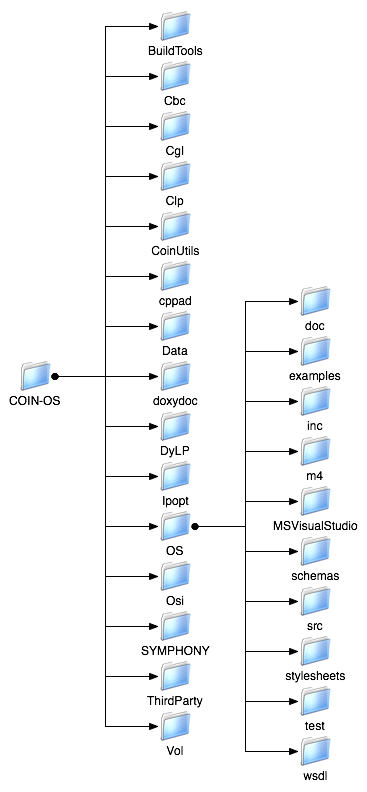
\includegraphics[scale=0.5]{\figurepath/OSProjectRootDirectory.png}
\caption{The OS project root directory.} 
\label{figure:osprojectrootdir}
\end{figure}

If you download the OS package, you get these additional COIN-OR projects. The links to the project home pages are provided below and give more information on these projects. 
\begin{itemize}
\item {\tt BuildTools} \url{projects.coin-or.org\BuildTools}
\item {\tt Cbc} \url{projects.coin-or.org\Cbc}
\item {\tt Clp}  \url{projects.coin-or.org\Clp}
\item {\tt CppAD} \url{projects.coin-or.org\CppAD}
\item {\tt Dylp} \url{projects.coin-or.org\Dylp}
\item {\tt Osi} \url{projects.coin-or.org\Osi}
\item {\tt SYMPHONY}   \url{projects.coin-or.org\SYMPHONY}
\end{itemize}

The following directories are also in the project root. 
\begin{itemize}
\item {\tt bin} after executing {\tt make install} the bin directory will contain {\tt OSSolverService}, {\tt clp}, {\tt cbc},  {\tt cbc-generic} and {symphony}.

\item {\tt Data} this directory contains numerous test problems that are used by some of the COIN-OR project's unitTest.

\item {\tt doxydoc} is a folder for documentation

\item {\tt include} is a directory for header files. If the user wishes to write code to link against any of the libraries in the {\tt lib} directory, it may be necessary to include these header files.

\item {\tt lib} is a directory of libraries. After running {\tt make install} the OS library along with all other COIN-OR libraries are installed in {\tt lib}.

\item {\tt ThirdParty} is a  directory for third party software. For example, if AMPL related software is used such as {\tt amplClient} is used, then certain AMPL libraries need to be present. This should go into the {\tt ASL} directory in {\tt ThirdParty.}
\end{itemize}




The directories in the OS directory are outlined in Figure \ref{figure:osdirectory}.


\begin{figure}
\centering
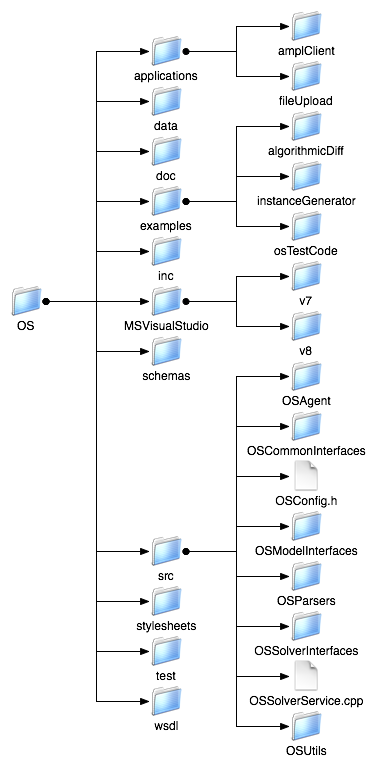
\includegraphics[scale=0.5]{\figurepath/OSDirectory.png}
\caption{The OS directory.} 
\label{figure:osdirectory}
\end{figure}

The OS directories include the following:

\begin{itemize}

\item {\tt data} is a directory that holds test problems. These test problems are used by the {\tt unitTest}. Many of these files are also used to illustrate how the {\tt OSSovlerService} works. See Section \ref{section:ossolverservice}.

\item {\tt doc} is the directory with documentation, include this {\it OS User's Manual.}

\item {\tt examples} is a directory with code examples that illustrate various aspects of the OS project.    These are described in Section \ref{section:examples}.

\item {\tt inc} is the directory with the config\_os.h file which has information about which projects are included in the distribution.

\item {\tt schemas} is the directory that contains the W3C XSD (see \url{www.w3c.org}) schemas that are behind the OS standards. These are described in more detail in Section \ref{section:schemadescriptions}.

\item {\tt src} is the directory with all of the source code for the OS Library and for the executable {\tt OSSolverService}. The OS Library components are described in Section \ref{section:oslibrary}.

\item {\tt stylesheets} this directory contains the XSLT stylesheet that is used to transform the solution instance in OSrL format into HTML so that it can be displayed in a browser.

\item {\tt test} this directory contains the {\tt unitTest}.


\item  {\tt wsdl} is a directory of WSDL (Web Services Discovery Language) files. These are used to specify the inputs and outputs for the methods provided by a Web service. The most relevant file for the current version of the OS project is {\tt OShL.wsdl}.  This describes the set of inputs and outputs for the methods implemented in the {\tt OSSolverService}. See Section \ref{section:ossolverservice}.
\end{itemize}




\subsection{Key Protocols}\label{section:schemadescriptions}

The objective of  (OS) is to provide a set of standards for representing optimization instances, results, solver options, and communication between clients and solvers in a distributed environment using Web Services.  These standards are specified by W3C XSD schemas. The schemas for the OS project are contained in the {\tt schemas} folder under the {\tt OS} root. There are numerous schemas in this directory that are part of the OS standard. For a full description of all the schemas see  Ma \cite{junma2005}.  We briefly discuss the standards most relevant to the current version of the OS project. 

\begin{itemize}


\item[] {\bf OSiL (Optimization Services instance Language):} an
XML-based language for representing instances of large-scale
optimization problems including linear programs, mixed-integer programs,
quadratic programs, and very general nonlinear programs.

     OSiL,  stores optimization problem instances as
XML files.  Consider the following problem instance that is a
modification of an example of Rosenbrock \cite{rosenbrock1960}:
%
\begin{alignat}{2}
& \mbox{Minimize} & \quad (1 - x_{0})^{2} + 100(x_{1} - x_{0}^{2})^{2} + 9x_{1} \label{eq:roobj}\\
& \mbox{Subject to} & \quad x_{0} + 10.5 x_{0}^{2} + 11.7 x_{1}^{2} + 3x_{0}x_{1}  &\le 25  \label{eq:ro1}\\
& & \ln(x_{0} x_{1}) + 7.5 x_{0} + 5.25 x_{1} &\ge 10 \label{eq:ro2}\\
& & x_{0}, x_{1} &\ge 0 \label{eq:ro3}
\end{alignat}


There are two continuous variables, $x_{0}$ and $x_{1}$, in this instance, each with a lower bound of 0. Figure~\ref{figure:variableselement} shows how we represent this information in an XML-based OSiL file.  Like all XML files, this is a text file that contains both {\it markup} and {\it data}. In this case there are two types of markup, {\it elements} (or {\it tags}\/) and {\it attributes} that describe the elements. Specifically, there are a {\tt <variables>} element and two {\tt <var>} elements. Each {\tt <var>}
element has attributes {\tt lb}, {\tt name}, and {\tt type} that
describe properties of a decision variable: its lower bound, ``name'', and
domain type.


\begin{figure}[b]
\centering
   \small {\obeyspaces\let =\
\fbox{\tt\begin{tabular}{@{}l@{}}
<variables numberOfVariables="2">\\[\Sb]
    <var lb="0" name="x0" type="C"/>\\[\Sb]
    <var lb="0" name="x1" type="C"/>\\[\Sb]
</variables>\\[\Sb]
\end{tabular} }} \medskip
\caption{The {\tt <variables>} element for the example (1)--(4).}\label{figure:variableselement}
\end{figure}


     To be useful for communication between solvers and modeling
languages, OSiL instance files must conform to a standard.
An XML-based representation standard is imposed
through the use of a {\em W3C XML Schema.} The W3C, or World Wide
Web Consortium (\url{www.w3.org}), promotes standards for
the evolution of the web and for interoperability between web
products.  XML Schema (\url{www.w3.org/XML/Schema}) is one
such standard.  A schema specifies the elements and attributes that
define a specific XML vocabulary. The W3C XML Schema is thus a schema
for schemas; it specifies the elements and attributes for a schema
that in turn specifies elements and attributes for an XML
vocabulary such as OSiL. An XML file that conforms to a
schema is called {\it valid} for that schema.  

     By analogy to object-oriented programming, a schema is akin to a header file in C++ that defines the members and methods in a class.  Just as a class in C++ very explicitly describes member and method names and properties, a
schema explicitly describes element and attribute names and properties.

{\small
\begin{figure}[b]
   \small {\obeyspaces\let =\
\makebox[0in][t]{\fbox{\tt\begin{tabular}{@{}l@{}}
<xs:complexType name="Variables">\\[\Sb]
    <xs:sequence>\\[\Sb]
        <xs:element name="var" type="Variable" maxOccurs="unbounded"/>\\[\Sb]
    </xs:sequence>\\[\Sb]
    <xs:attribute name="numberOfVariables"\\[\Sb]
            type="xs:positiveInteger" use="required"/>\\[\Sb]
</xs:complexType>\\[\Sb]
\end{tabular} }}} \medskip
\caption{The {\tt  Variables} complexType  in the OSiL
schema.}\label{figure:osilvariables}
\end{figure}
}%end small


{\small
\begin{figure}[b]
   \small {\obeyspaces\let =\
\makebox[0in][t]{\fbox{\tt\begin{tabular}{@{}l@{}}
<xs:complexType name="Variable">\\[\Sb]
    <xs:attribute name="name" type="xs:string" use="optional"/>\\[\Sb]
    <xs:attribute name="init" type="xs:string" use="optional"/>\\[\Sb]
    <xs:attribute name="type" use="optional" default="C">\\[\Sb]
        <xs:simpleType>\\[\Sb]
            <xs:restriction base="xs:string">\\[\Sb]
                <xs:enumeration value="C"/>\\[\Sb]
                <xs:enumeration value="B"/>\\[\Sb]
                <xs:enumeration value="I"/>\\[\Sb]
                <xs:enumeration value="S"/>\\[\Sb]
            </xs:restriction>\\[\Sb]
        </xs:simpleType>\\[\Sb]
    </xs:attribute>\\[\Sb]
    <xs:attribute name="lb" type="xs:double" use="optional" default="0"/>\\[\Sb]
    <xs:attribute name="ub" type="xs:double" use="optional" default="INF"/>\\[\Sb]
</xs:complexType>\\[\Sb]
\end{tabular} }}} \medskip
\caption{The {\tt  Variable} complexType in the OSiL
schema.}\label{figure:osilvar}
\end{figure}
} %end small



Figure ~\ref{figure:osilvariables} is a piece of our schema for OSiL. In W3C XML Schema jargon, it defines a {\it complexType,}  whose purpose is to specify elements and attributes that are allowed to appear in a valid XML instance file such as the one excerpted in Figure~\ref{figure:variableselement}. In particular, Figure~\ref{figure:osilvariables} defines the complexType named {\tt Variables}, which
comprises an element named {\tt <var>} and an attribute named {\tt
numberOfVariables}. The {\tt numberOfVariables} attribute is of a
standard type {\tt positiveInteger}, whereas the {\tt <var>} element is
a user-defined complexType named {\tt Variable}. Thus the complexType {\tt
Variables} contains a sequence of {\tt <var>} elements that
are of complexType {\tt Variable}. OSiL's schema must also provide a
specification for the {\tt Variable} complexType, which is shown in
Figure \ref{figure:osilvar}.

In OSiL the linear part of the problem is stored in the  {\tt
<linearConstraintCoefficients>} element, which stores the coefficient 
matrix using three arrays as proposed in the earlier LPFML schema
\cite{fourer2005a}.  There is a child element of {\tt
<linearConstraintCoefficients>} to represent each array: {\tt <value>} for an array of nonzero coefficients, {\tt <rowIdx>} or {\tt <colIdx>} for a corresponding array of row indices or column indices, and {\tt <start>} for an array that indicates where each row or column begins in the previous two arrays.


\begin{figure}[ht]
\centering
   \small {\obeyspaces\let =\
\fbox{\tt\begin{tabular}{@{}l@{}}
<linearConstraintCoefficients numberOfValues="3">\\[\Sb]
    <start>\\[\Sb]
        <el>0</el><el>2</el><el>3</el>\\[\Sb]
    </start>\\[\Sb]
    <rowIdx>\\[\Sb]
        <el>0</el><el>1</el><el>1</el>\\[\Sb]
    </rowIdx>\\[\Sb]
    <value>\\[\Sb]
        <el>1.</el><el>7.5</el><el>5.25</el>\\[\Sb]
    </value>\\[\Sb]
</linearConstraintCoefficients>\\[\Sb]
\end{tabular} }} \medskip\\[\Sb]
\caption{The {\tt <linearConstraintCoefficients>} element for constraints
(\ref{eq:ro1}) and (\ref{eq:ro2}).}\label{figure:rolistMatrix}
\end{figure}

The quadratic part of the problem is represented as follows.

\begin{figure}[ht]
\centering
   \small {\obeyspaces\let =\
\fbox{\tt\begin{tabular}{@{}l@{}}
<quadraticCoefficients numberOfQuadraticTerms="3">\\[\Sb]
     <qTerm idx="0" idxOne="0" idxTwo="0" coef="10.5"/>\\[\Sb]
     <qTerm idx="0" idxOne="1" idxTwo="1" coef="11.7"/>\\[\Sb]
     <qTerm idx="0" idxOne="0" idxTwo="1" coef="3."/>\\[\Sb]
</quadraticCoefficients>\\[\Sb]
\end{tabular} }} \medskip
\caption{The {\tt <quadraticCoefficients>} element for constraint (\ref{eq:ro1}).} 
\label{figure:qterms}
\end{figure}

The nonlinear part of the problem is given in Figure \ref{figure:roobjnlnode}.



{\small
\begin{figure}[t]
\centering
   \small {\obeyspaces\let =\
\fbox{\tt\begin{tabular}{@{}l@{}}
<nl idx="-1">\\[\Sb]
     <plus>\\[\Sb]
          <power>\\[\Sb]
               <minus>\\[\Sb]
                    <number value="1.0"/>\\[\Sb]
                    <variable coef="1.0" idx="0"/>\\[\Sb]
               </minus>\\[\Sb]
               <number value="2.0"/>\\[\Sb]
          </power>\\[\Sb]
          <times>\\[\Sb]
               <power>\\[\Sb]
                    <minus>\\[\Sb]
                         <variable coef="1.0" idx="0"/>\\[\Sb]
                         <power>\\[\Sb]
                              <variable coef="1.0" idx="1"/>\\[\Sb]
                              <number value="2.0"/>\\[\Sb]
                         </power>\\[\Sb]
                    </minus>\\[\Sb]
                    <number value="2.0"/>\\[\Sb]
               </power>\\[\Sb]
               <number value="100"/>\\[\Sb]
          </times>\\[\Sb]
     </plus>\\[\Sb]
</nl>\\[\Sb]
\end{tabular} }} \medskip\\[\Sb]
\caption{The {\tt <nl>} element for the nonlinear part of the objective (\ref{eq:roobj}).}\label{figure:roobjnlnode}
\end{figure}
}



 The complete OSiL representation is given in the Appendix.

\item[] {\bf OSrL (Optimization Services result Language):}  an
XML-based language for representing the solution of large-scale
optimization problems including linear programs, mixed-integer programs,
quadratic programs, and very general nonlinear programs.  As example solution (for the problem given in (\ref{eq:roobj})--(\ref{eq:ro3}) ) in OSrL format is given below. 

\begin{verbatim}
<?xml version="1.0" encoding="UTF-8"?>
<?xml-stylesheet type = "text/xsl" 
    href = "/Users/kmartin/Documents/files/code/cpp/OScpp/COIN-OSX/OS/stylesheets/OSrL.xslt"?>
<osrl xmlns="os.optimizationservices.org" xmlns:xsi="http://www.w3.org/2001/XMLSchema-instance"
    xsi:schemaLocation="os.optimizationservices.org http://www.optimizationservices.org/schemas/OSrL.xsd">
    <resultHeader>
        <generalStatus type="success"/>
        <serviceName>Solved using a LINDO service</serviceName>
        <instanceName>Modified Rosenbrock</instanceName>
    </resultHeader>
    <resultData>
        <optimization numberOfSolutions="1" numberOfVariables="2" numberOfConstraints="2"
            numberOfObjectives="1">
            <solution objectiveIdx="-1">
                <status type="optimal"/>
                <variables>
                    <values>
                        <var idx="0">0.87243</var>
                        <var idx="1">0.741417</var>
                    </values>
                    <other name="reduced costs" description="the variable reduced costs">
                        <var idx="0">-4.06909e-08</var>
                        <var idx="1">0</var>
                    </other>
                </variables>
                <objectives>
                    <values>
                        <obj idx="-1">6.7279</obj>
                    </values>
                </objectives>
                <constraints>
                    <dualValues>
                        <con idx="0">0</con>
                        <con idx="1">0.766294</con>
                    </dualValues>
                </constraints>
            </solution>
        </optimization>

\end{verbatim}




\item[] {\bf OSoL (Optimization Services option Language):}  an
XML-based language for representing options that get passed to an optimization solver. 

\item[] {\bf OSnL (Optimization Services nonlinear Language):}  The OSnL schema is imported by the OSiL schema and is used to represent the nonlinear part of an optimization instane. This is explained in greater detail in Section \ref{section:osexpressiontreeclass}. Also refer to Figue \ref{figure:roobjnlnode} for an illustration of elements from the OSnL standard. 



\item[]   {\bf OSpL (Optimization Services process Language):} is a standard for dynamic process information that is kept by the Optimization Services registry. 
It is the result of a {\tt knock} operation. See the example given in Section \ref{section:knock}.

\end{itemize}

\section{The OS Library Components}\label{section:oslibrary}

\subsection{OSAgent}\label{section:osagent}

The {\tt OSAgent}  part of the library is used to facilitate communication with remote solvers. It is not used if the solver is invoked locally (i.e. on the same machine). 

\subsection{OSCommonInterfaces}

Mention the OSnL node class. List which NL operators can be used.

\subsubsection{The OSInstance Class}\label{section:osinstanceclass}

\subsubsection{The OSExpressionTree OSnLNode Classes}\label{section:osexpressiontreeclass}

The {\tt OSExpressionTree} class provides the in-memory representation of the nonlinear terms.  Our design goal is  to allow for efficient parsing of OSiL instances, while providing an API that meets the needs of diverse solvers.  Conceptually, any nonlinear expression in the objective or constraints is represented by a tree.  The expression tree for the nonlinear part of the objective function (\ref{eq:roobj}), for example, has the form illustrated in Figure~\ref{figure:expressiontree}.  The choice of a data structure to store such a tree --- along with the associated methods of an API --- is a key aspect in the design of the {\tt OSInstance} class. 

\begin{figure}[ht]
\centering
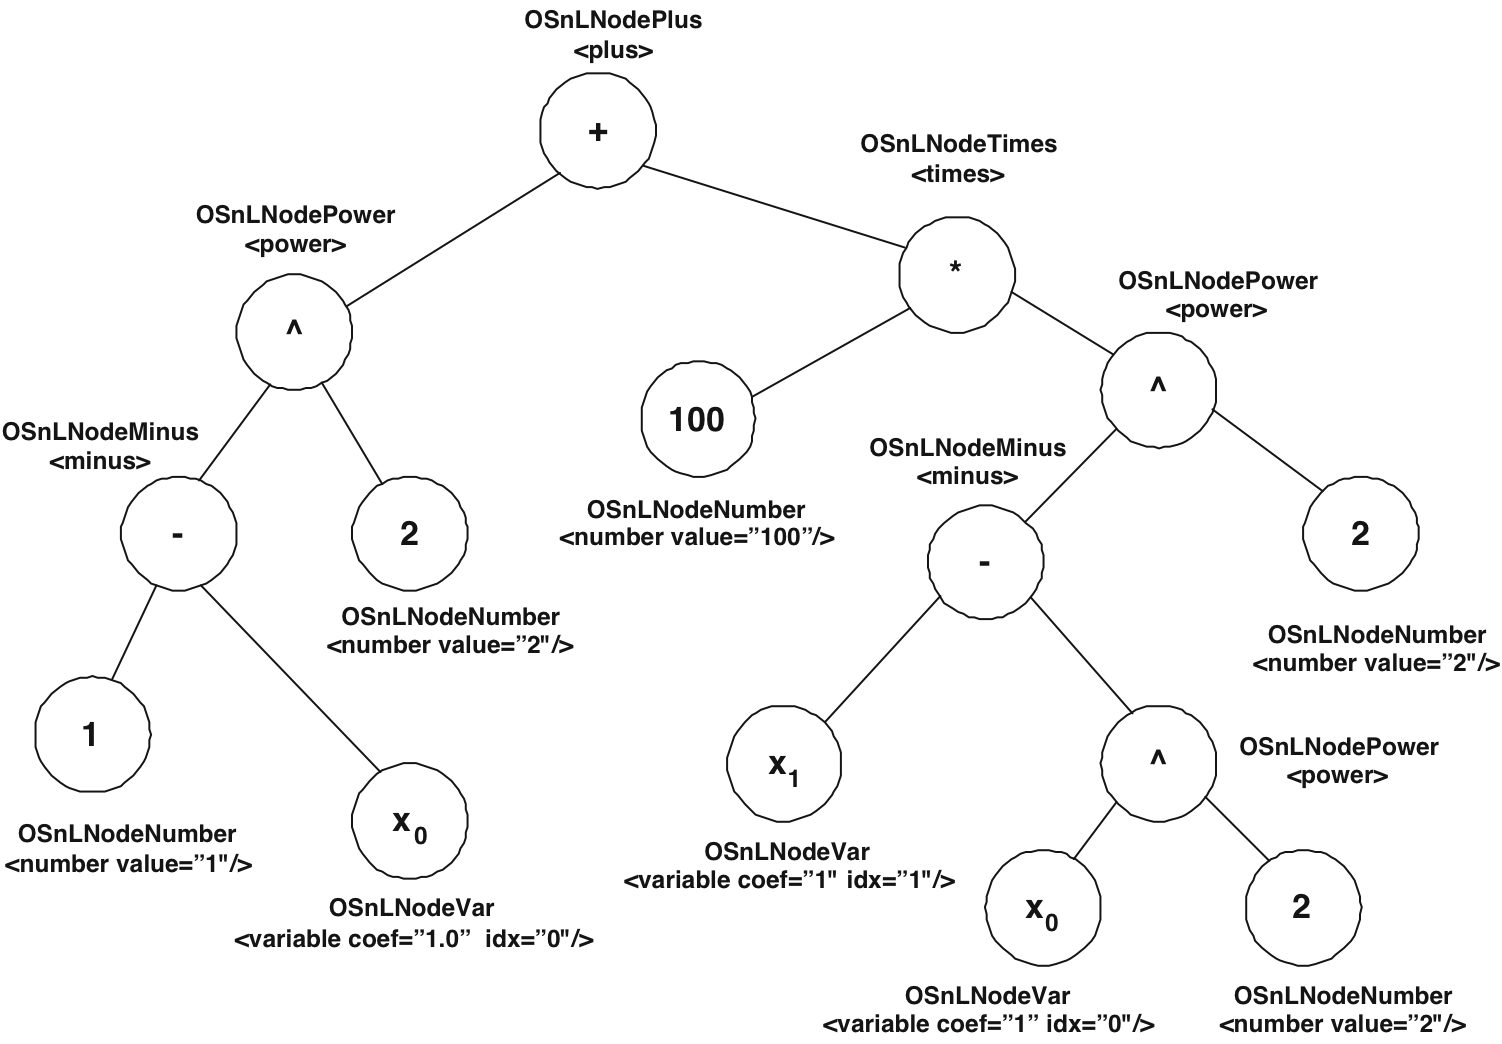
\includegraphics[%
  scale=0.38]{\figurepath/expressiontree.png}
\caption{Conceptual expression tree for the nonlinear part of the objective (\ref{eq:roobj}).} \label{figure:expressiontree}
\end{figure}
  

A base abstract class {\tt OSnLNode} is defined and  all of an OSiL file's
operator and operand elements used in defining a
nonlinear expression are extensions of the base element type {\tt OSnLNode}. There is an element type {\tt OSnLNodePlus}, for example, that
extends {\tt OSnLNode}; then in an OSiL instance
file, there are {\tt <plus>} elements that are of type {\tt
OSnLNodePlus}.   Each {\tt OSExpressionTree} object contains a pointer to an {\tt OSnLNode} object that is the root of the corresponding expression tree.  To every element that extends the {\tt OSnLNode} type in an OSiL instance file, there corresponds a class that derives from the {\tt OSnLNode} class in an {\tt OSInstance} data structure.  Thus we can construct an expression tree of homogenous nodes, and methods that operate on the expression tree to calculate function values, derivatives, postfix notation, and the like do not require switches or complicated logic.


\begin{figure}[ht]
\centering
   \small {\obeyspaces\let =\
\fbox{\tt\begin{tabular}{@{}l@{}}
   double OSnLNodePlus::calculateFunction(double *x)\{\\[\Sb]
      m\_dFunctionValue = \\[\Sb]
         m\_mChildren[0]->calculateFunction(x) +\\[\Sb]
         m\_mChildren[1]->calculateFunction(x);\\[\Sb]
      return m\_dFunctionValue;\\[\Sb]
   \} //calculateFunction\\[\Sb]
\end{tabular} }} \medskip
\caption{The function calculation method for the ``plus'' node class with polymorphism}
   \vspace{-8pt} \label{figure:calcfunction}
\end{figure}


    The {\tt OSInstance} class has a variety of {\tt calculate()} methods, based on two pure virtual functions in the {\tt OSInstance} class.  The first of these, {\tt calculateFunction()}, takes an array of {\tt double} values corresponding to decision variables, and evaluates the expression tree for those values.  Every class
that extends {\tt OSnLNode} must implement this method.  As an example, the {\tt calculateFunction} method for the {\tt OSnLNodePlus} class is shown in Figure \ref{figure:calcfunction}.  Because the OSiL instance file must be validated against its schema, and in the schema each {\tt <OSnLNodePlus>} element is specified to have exactly two child elements, this {\tt calculateFunction} method can assume that there are
exactly two children of the node that it is operating on.  Thus through the use of polymorphism and recursion the need for switches like those in Figure~\ref{figure:parsecode1} is eliminated. This design makes adding new operator elements easy; it is simply a matter of adding a new class and implementing the {\tt
calculateFunction()} method for it.



The following {\tt  OSnLNode} classes are currently supported.

\begin{itemize}
\item OSnLNodeVariable
\item OSnLNodeTimes 
\item OSnLNodePlus 
\item OSnLNodeSum 
\item OSnLNodeMinus 
\item OSnLNodeNegate
\item OSnLNodeDivide 
\item OSnLNodePower 
\item OSnLNodeProduct
\item OSnLNodeLn 
\item OSnLNodeSqrt 
\item OSnLNodeSquare
\item OSnLNodeSin
\item OSnLNodeCos
\item OSnLNodeExp
\item OSnLNodeif
\item OSnLNodeAbs
\item OSnLNodeMax
\item OSnLNodeMin
\item OSnLNodeE
\item OSnLNodePI
\item OSnLNodeAllDiff
\end{itemize}





\subsection{OSModelInterfaces}\label{section:osmodelinterfaces}





\subsection{OSParsers}



\subsection{OSSolverInterfaces}


The {\tt OSSolverInterfaces} library is designed to facilitate linking the OS library with various solver APIs. We first describe how to take a problem instance in OSiL format and connect to a solver that has a COIN-OR OSI interface.  See the OSI project \url{www.projects.coin-or.org/Osi}.   We then describe hooking to the COIN-OR nonlinear code {\tt Ipopt.} See \url{www.projects.coin-or.org/Ipopt}.  Finally we describe hooking to two commercial solvers KNITRO and LINDO. 

The OS library has been tested with the following solvers using the Osi Interface.

\begin{itemize}
\item Cbc
\item Clp
\item Cplex
\item DyLP
\item Glpk
\item SYMPHONY
\end{itemize}

In the {\tt OSSolverInterfaces} library there is an abstract class {\tt DefaultSolver} that has the following key members:

\begin{verbatim}
std::string osil;
std::string osol;
std::string osrl;
OSInstance *osinstance;
OSResult  *osresult;
\end{verbatim}
and the pure virtual function
\begin{verbatim}
virtual void solve() = 0 ;	
\end{verbatim}
In order to use a solver through the COIN-OR {\tt Osi} interface it is necessary to an object in the {\tt CoinSolver} class which inherits from the {\tt DefaultSolver} class and implements the appropriate {\tt solve()} function.  We illustrate with the Clp solver.

\begin{verbatim}
DefaultSolver *solver  = NULL;
solver = new CoinSolver();
solver->m_sSolverName = "clp";
\end{verbatim}

Assume that the data file containing the problem has been read into the string {\tt osil} and the solver options are in the string {\tt osol}. Then the {\tt Clp} solver is invoked as follows.

\begin{verbatim}
solver->osil = osil;
solver->osol = osol;
solver->solve();
\end{verbatim}

Finally, get the solution in {\tt OSrL} format as follows

\begin{verbatim}
cout << solver->osrl << endl;
\end{verbatim}

Even though LINDO and KNITRO are commercial solvers and do not have a COIN-OR {\tt Osi} interface these solvers are used in exactly the same manner as a COIN-OR solver. For example, to invoke the LINDO solver we do the following.

\begin{verbatim}
solver = new LindoSolver();	
\end{verbatim}

Similarly for KNITRO and Ipopt. In the case of the KNITRO, the {\tt KnitroSolver} class inherits from both {\tt DefaultSolver} class and the KNITRO {\tt NlpProblemDef} class. See \url{Kipp -- put in Knitro manual link} for more information on the KNITRO solver C++ implementation and the {\tt NlpProblemDef} class. Similarly, for Ipopt the {\tt IpoptSolver} class inherits from both the  {\tt DefaultSolver} class and the Ipopt {\tt TNLP} class.  See \url{Kipp -- put in Ipopt manual link} for more information on the Ipopt solver C++ implementation and the {\tt TNLP} calss.

In the examples above the problem instance was assumed to be read from a file into the string {\tt osil} and then into the class member {\tt solver->osil.} However, everything can be done entirely in memory. For example, it is possible to use the {\tt OSInstance} class to create an in-memory problem representation and give this representation directly to a solver class that inherits from {\tt DefaultSolver}. The class member to use is {\tt osinstance.} This is illustrated in the example given in Section \ref{subsection:exampleOSInstance}.


\subsection{OSUtils}

\section{The  OSInstance API}\label{section:osinstance}

\subsection{Get Methods}

Don't forget to mention getting prefix an postfix. Illustrate some of this like in the unitTest.

\subsection{Set Methods}

\subsection{Calculate Methods}

\section{Hooking to An Algorithmic Differentiation Package}\label{section:ad}

\section{The OSSolverService}\label{section:ossolverservice}

The {\tt OSSolverService} is a command line executable designed to pass problem instances in either  OSiL, AMPL nl, or MPS format  to solvers and get the optimization result back to be displayed either to standard output or a specified browser.  The {\tt OSSovlerService} can be used to invoke a solver locally or on a remote server. It can work either synchronously or asynchronously. 

\subsection{OSSolverService Input Parameters}

At present, the {\tt OSSolverService} takes the following parameters. The order of the parameters is irrelevant.  Not all the parameters are required. However, if the {\tt solve} or {\tt send} service methods are invoked a problem instance location must be specified. 

\begin{itemize}

\item[] {\bf -osil xxx.osil}  this is the name of the file that contains the optimization instance in OSiL format. It is assumed that this file is available in a directory on the machine that is running {\tt OSSolverService}. If this option is not specified then the instance location must be specified in the OSoL solver options file.

\item[] {\bf -osol xxx.osol}  this is the name of the file that contains the solver options. It is assumed that this file is available in a directory on the machine that is running {\tt OSSolverService}. It is not necessary to specify this option.

\item[] {\bf -osrl xxx.osrl}  this is the name of the file that contains the solver solution. A valid file path must be given on the machine that is running {\tt OSSolverService}. It is not necessary to specify this option.

\item[] {\bf -serviceLocation}  is the URL of the solver service. This is not required, and if not specified it is assumed that the problem is solved locally. 

\item[] {\bf -serviceMethod  method}  this is  the solver service required. The options are {\tt solve}, {\tt send},{\tt kill},{\tt knock}, {\tt getJobID}, and {\tt retrieve}. The use of these options is illustrated in the examples below. This option is not required, and the default value is {\tt solve.}

\item[] {\bf -mps  xxx.mps}  this is the name of the mps file if the problem instance is in mps format. It is assumed that this file is available in a directory on the machine that is running {\tt OSSolverService}. The default file format is OSiL so this option is not required.

\item[] {\bf -nl  xxx.nl}  this is the name of the AMPL nl file if the problem instance is in AMPL nl  format. It is assumed that this file is available in a directory on the machine that is running {\tt OSSolverService}. The default file format is OSiL so this option is not required.

\item[] {\bf -solver  solverName}  Possible values for default OS installation are {tt clp} (COIN-OR Clp), {\tt cbc} (COIN-OR Cbc), {\tt dylp} (COIN-OR DyLP), and {\tt symphony} (COIN-OR SYMPHONY). Other solvers supported (if the necessary libraries are present) are {\tt cplex} (Cplex through COIN-OR Osi), {\tt glpk} (glpk through COIN-OR Osi), {\tt ipopt} (COIN-OR Ipopt),  {\tt knitro} (Knitro), and {\tt lindo} {\tt LINDO}. If no value is specified for this parameter, then {\tt cbc} is the default value of this parameter if the the {\tt solve} or {\tt send} service methods are used.


\item[] {\bf -browser  browserName} this paramater is a path to the browser on the local machine. If this optional parameter is specified then the solver result in OSrL format is transformed using XSLT into HTML and displayed in the browser. 

\item[] {\bf -config pathToConfigureFile} this parameter specifies a path on the local machine to a text file containing values for the input parameters. This is convenient for the user not wishing to constantly retype parameter values.

\end{itemize}



The input parameters to the {\tt OSSolverService} may be given entirely in the command line or in a configuration file.  We first illustrate giving all the  parameters in the command line. The following command will invoke the {\tt Clp} solver on the local machine to solve the problem instance {\tt parincLinear.osil}.

\begin{verbatim}
OSSolverService -solver clp -osil ../data/parincLinear.osil 
\end{verbatim}

Alternatively, these parameters can be put into a configuration file. Assume that the configuration file of interest is {\tt testlocalclp.config}. It would contain the two lines of information
\begin{verbatim}
-osil ../data/parincLinear.osil
-solver clp
\end{verbatim}
Then the command line is
\begin{verbatim}
OSSolverService -config ../data/testlocalclp.config
\end{verbatim}


{\bf Some Rules:}

\begin{itemize}
\item[1.]  When using the {\tt send()} or  {\tt solve()} methods a problem instance file location {\it must} be specified either at  the command line, in the configuration file, or in the {\tt <instanceLocation>} element in the OSoL options file file.

\item[2.]  The default {\tt serviceMethod} is {\tt solve} if another service method is not specified.   The service method cannot be specified in the OSoL options file. 

\item [3.]  If the {\tt solver} option is not specified, the COIN-OR solver {\tt Cbc} is the default solver used. In this case an error is thrown if the problem instance has quadratic or other nonlinear terms. 

\item[4.]  If the options {\tt send}, {\tt kill}, {\tt knock},  {\tt getJobID},  or {\tt retrieve} are specified, a  {\tt serviceLocation} must be specified. 

\end{itemize}



Parameters specified in the configure file are overridden by parameters specified at the command line. This is convenient if a user has a base configure file and wishes to override only a few options. For example,
\begin{verbatim}
OSSolverService -config ../data/testlocalclp.config -solver lindo
\end{verbatim}
or
\begin{verbatim}
OSSolverService -solver lindo -config ../data/testlocalclp.config 
\end{verbatim}
will result in the LINDO solver being used even though Clp is specified in the {\tt testlocalclp} configure file.



\subsection{Solving Problems Locally}

Generally, when solving a problem locally the user will use the {\tt solve} service method. The {\tt solve} method is invoked synchronously and waits for the solver to return the result.  This is illustrated in Figure \ref{figure:ossolverservice}. As illustrated, the {\tt OSSolverService} reads a file on the hard drive with the optimization instance, usually in OSiL format. The optimization instance is parsed into a string which is passed to the {\tt OSLibrary} which is linked with various solvers. The result of the optimization is passed back to the {\tt OSSolverService} as a string in OSrL format.  



\begin{figure}
\centering
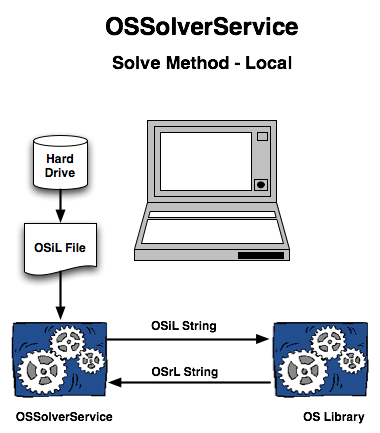
\includegraphics[scale=0.5]{\figurepath/OSSolverServiceLocal.png}
\caption{A local call to {\tt solve}.} 
\label{figure:ossolverservicelocal}
\end{figure}



Here is an example of using a configure file,  {\tt testlocal.config}, to invoke {\tt Ipopt} locally using the {\tt solve} command.

\begin{verbatim}
-osil ../data/parincQuadratic.osil
-solver ipopt
-serviceMethod solve
-browser /Applications/Firefox.app/Contents/MacOS/firefox
-osrl /Users/kmartin/temp/test.osrl
\end{verbatim}



The first line of {\tt testlocal.config} gives the local location of the OSiL file, {\tt parincQuadratic.osil}, that contains the problem instance. The second parameter, {\tt -solver ipopt},  is the solver to be invoked, in this case COIN-OR Ipopt. The third parameter {\tt -serviceMethod solve} is not really needed, but included only for illustration. The default  solver service is {\tt solve.}  The fourth parameter is the location of the browser on the local machine. It will read the OSrL file on the local machine using the path specified by the value of the {\tt osrl} parameter, in this case {\tt /Users/kmartin/temp/test.osrl.}

Parameters may also be contained in an XML-file in OSoL format. In the configuration file {\tt testlocalosol.config} we illustrate specifying the instance location in an OSoL file.
\begin{verbatim}
-osol ../data/demo.osol
-solver clp
\end{verbatim}
The file {\tt demo.osol} is

\begin{verbatimtab}[4]
<?xml version="1.0" encoding="UTF-8"?>
<osol xmlns="os.optimizationservices.org">
	<general>         
		<instanceLocation locationType="local">
			../data/parincLinear.osil
		</instanceLocation>
	</general>
</osol>
\end{verbatimtab}

\subsection{Solving Problems Remotely with Web Services}

In many cases the client machine may be a ``weak client'' and  using a more powerful machine to solve a hard optimization instance is required. Indeed, one of the major purposes of Optimization Services is to facilitate optimization in a distributed environment.   We now provide examples that illustrate using the {\tt OSSolverService} executable to call a remote solver service.   By remote solver service we mean a solver service that is called using Web Services.  The OS implementation  of the solver service  uses Apache Tomcat. See \url{tomcat.apache.org}. The Web Service running on the server is a Java program based on Apache Axis. See \url{ws.apache.org/axis}. This is described in greater detail in Section \ref{section:tomcat}.  This Web Service is called {\tt OSSolverService.jws}. It is not necessary to use the Tomcat/Axis combination.



See Figure \ref{figure:ossolverservice} for an illustration of this process. The client machine uses {\tt OSSolverService} executable to call one of the six service methods, e.g. {\tt solve}. The  information such as the problem instance in OSiL format and solver options in OSoL format are packaged into a SOAP envelope and sent to the server. The server is running the Java Web Service {\tt OSSolverService.jws}. This Java program running in the Tomcat Java Servlet container implements the six service methods. If a {\tt solve} or {\tt send} request is sent to the server from the client, an optimization problem must be solved. The Java solver service solves the optimization instance by  calling the  OSSolverService on the server. So there is an OSSolverService on the client that calls the Web Service {\tt  OSSolverService.jws} that in turn calls  the executable {\tt OSSovlerService} on the server. The Java solver service passes options to the local {\tt OSSolverService} such as where the OSiL file is located and where to write the solution result.

\begin{figure}
\centering
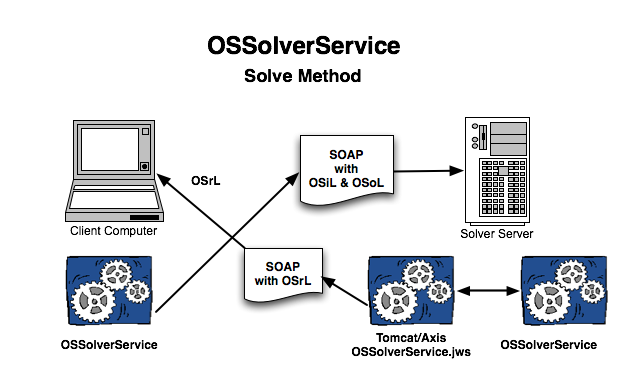
\includegraphics[scale=0.5]{\figurepath/OSSolverService.png}
\caption{A remote call to {\tt solve}.} 
\label{figure:ossolverservice}
\end{figure}


In the following sections we illustrate each of the six service methods.

\subsubsection{The  {\tt solve} Service Method}\label{section:solve}

First we illustrate a simple call to   {\tt OSSolverService.jws} and request a solution using the COIN-OR  {\tt Clp} solver.  The call on the client machine is

\begin{verbatim}
OSSolverService -config ../data/testremote.config
\end{verbatim}
where the {\tt testremote.config} file is
\begin{verbatim}
-osil ../data/parincLinear.osil
-serviceLocation http://128.135.130.17:8080/os/OSSolverService.jws
\end{verbatim}

No solver is specified so by default the  {\tt Cbc} solver will be used on the server.  

Now use an OSoL options file
\begin{verbatim}
OSSolverService -osol ../data/remoteSolve1.osol -osil ../data/parincLinear.osil
\end{verbatim}
where {\tt remoteSolve1.osol} is
\begin{verbatim}
<?xml version="1.0" encoding="UTF-8"?>
<osol xmlns="os.optimizationservices.org">
    <general>
        <serviceURI>http://128.135.130.17:8080/os/OSSolverService.jws</serviceURI>
    </general>
    <optimization>
    	<other name="os_solver">clp</other>
    </optimization>
</osol>
\end{verbatim}
In this case we specify a sover to use, name {\tt Clp}.

Next we illustrate a call to the remote SolverService and specify an OSiL instance that is on the remote machine.
\begin{verbatim}
OSSolverService -osol ../data/remoteSolve2.osol
\end{verbatim}
where the {\tt remoteSolve2.osol} file is
\begin{verbatimtab}[4]
<?xml version="1.0" encoding="UTF-8"?>
<osol xmlns="os.optimizationservices.org">
    <general>
        <serviceURI>http://128.135.130.17:8080/os/OSSolverService.jws</serviceURI>
         <instanceLocation locationType="local">
	 /home/kmartin/files/code/OSRepository/linear/continuous/pilot.osil
	 </instanceLocation>
    </general>
    <optimization>
    	<other name="os_solver">clp</other>
    </optimization>
</osol>
\end{verbatimtab}


If we were to change to the {\tt locationType} attribute in the {\tt <instanceLocation>} element to {\tt http} then we could specify the intance location to on yet another machine. This is illustrated below  for {\tt remoteSovle3.osol}.  The scenario is depicted in Figure \ref{figure:ossolverservice2}.  The OSiL string passed from the client to the solver service is empty.  However, the OSoL element {\tt <instanceLocation>}  has an attribute {\tt locationType} equal to   {\tt http}.  In this case, the text of the {\tt <instanceLoction>} element contains the URL of a third machine which has the problem intance {\tt parincLinear.osil}.  The solver service will contact the machine with URL {\tt gsbkip.chicagogsb.edu} and download this test problem. 
\begin{verbatimtab}[4]
<?xml version="1.0" encoding="UTF-8"?>
<osol xmlns="os.optimizationservices.org">
    <general>
        <serviceURI>http://128.135.130.17:8080/os/OSSolverService.jws</serviceURI>
         <instanceLocation locationType="http">
	 http://gsbkip.chicagogsb.edu/testproblems/parincLinear.osil
	 </instanceLocation>
    </general>
    <optimization>
    	<other name="os_solver">clp</other>
    </optimization>
</osol>
\end{verbatimtab}

\begin{figure}
\centering
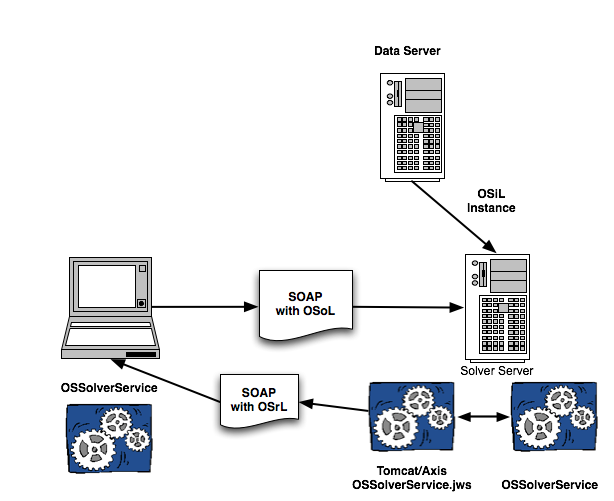
\includegraphics[scale=0.5]{\figurepath/OSSolverService2.png}
\caption{Downloading the instance from a remote source.} 
\label{figure:ossolverservice2}
\end{figure}

\subsubsection{The  {\tt send} Service Method}\label{section:send}

When the {\tt solve} service method is used, the {\tt OSSolverService} does not finish execution until the solution is returned from the remote solver service. The {\tt solve} method communicates synchronously with the remote solver service. This may not be desirable for large problems when the user does not want to wait for a response. The {\tt send} service method should be used when asynchronous communication is desired. When the send method is used the instance is communicated to the remote service and the {\tt OSSolverService} terminates after submission. An example of this is
\begin{verbatim}
OSSolverService -config ../data/testremoteSend.config
\end{verbatim}
where the {\tt testremoteSend.config} file is
\begin{verbatim}
-nl ../data/hs71.nl
-serviceLocation http://128.135.130.17:8080/os/OSSolverService.jws
-serviceMethod send
\end{verbatim}
In this example the COIN-OR {\tt Ipopt} solver is specified. The input file {\tt hs71.nl} is in AMPL format. Before sending this to the remote solver service the {\tt OSSolverService} executable converts  the nl format into the OSiL XML format and packages this into the SOAP envelope used by Web Services. 

Since the {\tt send} method involves asynchronous communication the remote solver service must keep track of jobs. The send methd requires a {\tt JobID}. In the above example  no {\tt JobID} was specified. When no {\tt JobID} is specified the {\tt OSSolverService} method first invokes the {\tt getJobID} service method to get a {\tt JobID} and then puts this information into a created OSoL file and send the information to the server. More information on the {\tt getJobID} service method is provided in Section \ref{section:getjobid}.  The {\tt OSSolverService} prints the OSoL file to standard output before termination. This is illustrated below,
\begin{verbatimtab}[4]
<?xml version="1.0" encoding="UTF-8"?> 
<osol xmlns="os.optimizationservices.org">
	<general> 
		<jobID>
		gsbrkm4__127.0.0.1__2007-06-16T15.46.46.075-05.00149771253
		</jobID>
	</general>
    <optimization>
    	<other name="os_solver">ipopt</other>
    </optimization>
</osol>
\end{verbatimtab}
The {\tt JobID} is one that is randomly generated by the server and passed back to the {\tt OSSolverService.} The user can also provide a {\tt JobID} in their OSoL file. For example, below is a user-provided OSoL file that could be specified in a configuration file or on the command line.
\begin{verbatimtab}[4]
<?xml version="1.0" encoding="UTF-8"?>
<osol xmlns="os.optimizationservices.org">
	<general>  
		<jobID>123456abcd</jobID>       
	</general>
    <optimization>
    	<other name="os_solver">ipopt</other>
    </optimization>
</osol>
\end{verbatimtab}

In order to be of any use, it is necesary to get the result of the optimization. This is described in Section \ref{section:retrieve}. Before proceeding to this section, we describe two ways for knowing when the optimization is complete. One feature of the standard OS remote SolverService is the ability to send an email when the job is complete. Below is an example of the {\tt OSoL} that uses the email feature.
\begin{verbatimtab}[4]
<?xml version="1.0" encoding="UTF-8"?>
<osol xmlns="os.optimizationservices.org">
 	<general>  
 		<jobID>123456abcd</jobID>   
 		<contact transportType="smtp">
			kipp.martin@chicagogsb.edu
		</contact>     
	</general>
    <optimization>
    	<other name="os_solver">lindo</other>
    </optimization>
</osol>
\end{verbatimtab}

The remote Solver Service will send an email to the above address when the job is complete. A second option for knowing when a job is complete is to use the knock method. 

Note that in all of these examples we provided a value for the {\tt name} attribute in the {\tt <other>} element. The remote solver service will use Cbc if another solver is not specified. 



\subsubsection{The  {\tt retrieve} Service Method}\label{section:retrieve}

The {\tt retrieve} has a single string argument which is an OSoL instance. Here is an example of using the {\tt retrieve} method with {\tt OSSolverService}.
\begin{verbatim}
OSSolverService -config ../data/testremoteRetrieve.config
\end{verbatim}
The {\tt testremoteRetrieve.config} file is
\begin{verbatim}
-serviceLocation http://128.135.130.17:8080/os/OSSolverService.jws
-osol ../data/retrieve.osol
-serviceMethod retrieve
-osrl /home/kmartin/temp/test.osrl
\end{verbatim}
and the {\tt retrieve.osol} file is
\begin{verbatimtab}[4]
<?xml version="1.0" encoding="UTF-8"?>
<osol xmlns="os.optimizationservices.org">
 	<general>         
 		<jobID>123456abcd</jobID>  
	</general>
</osol>
\end{verbatimtab}
The OSoL file {\tt retrieve.osol} contains a tag {\tt <jobID>} that is communicated to the remote service. The remove service locates the result returns it as a string. The string that is returned is an OSrL instance. 

\subsubsection{The  {\tt getJobID} Service Method}\label{section:getjobid}

Before  submitting a job with the {\tt send} method a {\tt JobID} is required. The {\tt OSSolverService} can get a {\tt JobID} as follows
\begin{verbatim}
-serviceLocation http://128.135.130.17:8080/os/OSSolverService.jws
-serviceMethod getJobID
\end{verbatim}
Note that no OSoL input file is specified. In this case, the {\tt OSSolverService} sends an empty string. A string is returned with the {\tt JobID}. This {\tt JobID} is then put into a {\tt <jobID>} element in an OSoL string that would be used by the {\tt send} method.


\subsubsection{The  {\tt knock} Service Method}\label{section:knock}

The OSSolverService terminates after executing the {\tt send} method. Therefore, it is necessary to know when the job is completed on the remote server. One way is to include an email address in the  {\tt <contact>}  element with the attribute {\tt transportType}     set to {\tt smtp}.  This was illustrated in Section \ref{section:solve}.  A second way to check on the status of a job is to use the {\tt knock} service method.  For example, assume a user   wants to know if  the job with {\tt JobID 123456abcd}  is complete. A user would make the request
\begin{verbatim}
OSSolverService -config ../data/testRemoteKnock.config
\end{verbatim}
where the {\tt testRemoteKnock.config} file is
\begin{verbatim}
-serviceLocation http://128.135.130.17:8080/os/OSSolverService.jws
-osplInput ../data/demo.ospl
-osol ../data/retrieve.osol
-serviceMethod knock
\end{verbatim}
the {\tt demo.ospl} file is
\begin{verbatim}
<?xml version="1.0" encoding="UTF-8"?>
<ospl xmlns="os.optimizationservices.org">
<processHeader>
<request action="getAll"/>
</processHeader>
<processData/>
</ospl>
\end{verbatim}
and the {\tt retrieve.osol} file is
\begin{verbatim}
<?xml version="1.0" encoding="UTF-8"?>
<osol xmlns="os.optimizationservices.org">
 	<general>         
 		<jobID>123456abcd</jobID>  
	</general>
</osol>
\end{verbatim}
The result of this request is a string in OSrL format.  Part of the return format is illustrated below.
\begin{verbatimtab}[4]
<jobs>
	<job jobID="123456abcd">
		<state>finished</state>
		<serviceURI>http://128.135.130.17:8080/ipopt/IPOPTSolverService.jws</serviceURI>
		<submitTime>2007-06-16T14:57:36.678-05:00</submitTime>
		<startTime>2007-06-16T14:57:36.678-05:00</startTime>
		<endTime>2007-06-16T14:57:39.404-05:00</endTime>
		<duration>2.726</duration>
 </job>
</jobs>
\end{verbatimtab}
Notice the {\tt <state>} element indicating that the job is finished.   

When making a {\tt knock} request,  the OSoL string can be empty. In this example, if the OSoL string had been empty the status of all jobs kept in the file ospl.xml is reported.  In our default solver service implementation, there is a configuration file {\tt OSParameter} that has a parameter {\tt MAX\_JOBIDS\_TO\_KEEP }.  The current default setting is 100.  In a large-scale or commercial implementation it might be wise to keep problem results and statistics in a database.  Also, there are values other than {\tt getAll} for the OSpL {\tt action} attribute in the {\tt <request>} tag.  For example, the {\tt action} can be set to a value of {\tt ping} if the user just wants to check if the remote solver service is up and running. 



\subsubsection{The  {\tt kill}   Service Method}

If the user submits a job that is taking too long or is a mistake it is possible to kill the job on the remote server using the {\tt kill} service method. For example to kill job {\tt 123456abcd} .  At the command line type
\begin{verbatim}
OSSolverService -config  ../data/kill.config
\end{verbatim}
where the configure file {\tt kill.config} is
\begin{verbatim}
-osol ../data/kill.osol
-serviceLocation http://128.135.130.17:8080/os/OSSolverService.jws
-serviceMethod kill
\end{verbatim}
and the {\tt kill.osol} file is
\begin{verbatimtab}[4]
<?xml version="1.0" encoding="UTF-8"?>
<osol xmlns="os.optimizationservices.org">
 	<general>         
 		<jobID>123456abcd</jobID>  
	</general>
</osol>
\end{verbatimtab}


\subsubsection{Summary}

Below is a summary of the inputs and outputs of the six service methods. See also Figures \ref{figure:async1} and \ref{figure:async2}.

\begin{itemize}
\item {\tt solve(osil, osol):}

\begin{itemize}

\item Inputs: a string with the instance in OSiL format and a string with the solver options in OSoL format

\item  Returns: a string with the solver solution in OSrL format

\item  Synchronous call, blocking request/response

\end{itemize}



\item {\tt send(osil, osol)}


\begin{itemize}

\item Inputs: a string with the instance in OSiL format and a string with the solver options in OSoL format

\item Returns:  a boolean, true if the problem was successfully submitted, false otherwise

\item Has the same signature as {\tt solve}

\item  Asynchronous (server side), non-blocking call

\item The {\tt osol} string should have a {\tt JobID} in the {\tt <jobID>} element
\end{itemize}

\item {\tt getJobID( osol)}

\begin{itemize}

\item Inputs: a string  with the solver options in OSoL format (in this case, the string may be empty because no options are required to get the JobID)

\item  Returns: a string which is the unique job id generated by the solver service

\item  Used to maintain session and state on a distributed system
\end{itemize}



\item {\tt knock(ospl, osol)}

\begin{itemize}

\item Inputs: a string in OSpL format and a string with the solver options in OSoL format

\item  Returns: process and job status information from the remote server in OSpL format

\end{itemize}

\item {\tt retrieve( osol)}


\begin{itemize}

\item Inputs: a string with the solver options  in OSoL format  

\item Returns: a string with the solver solution in OSrL format

\item The {\tt osol} string should have a {\tt JobID} in the {\tt <jobID>} element

\end{itemize}

\item {\tt kill( osol)}


\begin{itemize}

\item Inputs: a string with the solver options  in OSoL format  

\item  Returns: process and job status information from the remote server in OSpL format

\item  Critical in long running optimization jobs

\end{itemize}

\end{itemize}



\begin{figure}[ht]
\centering
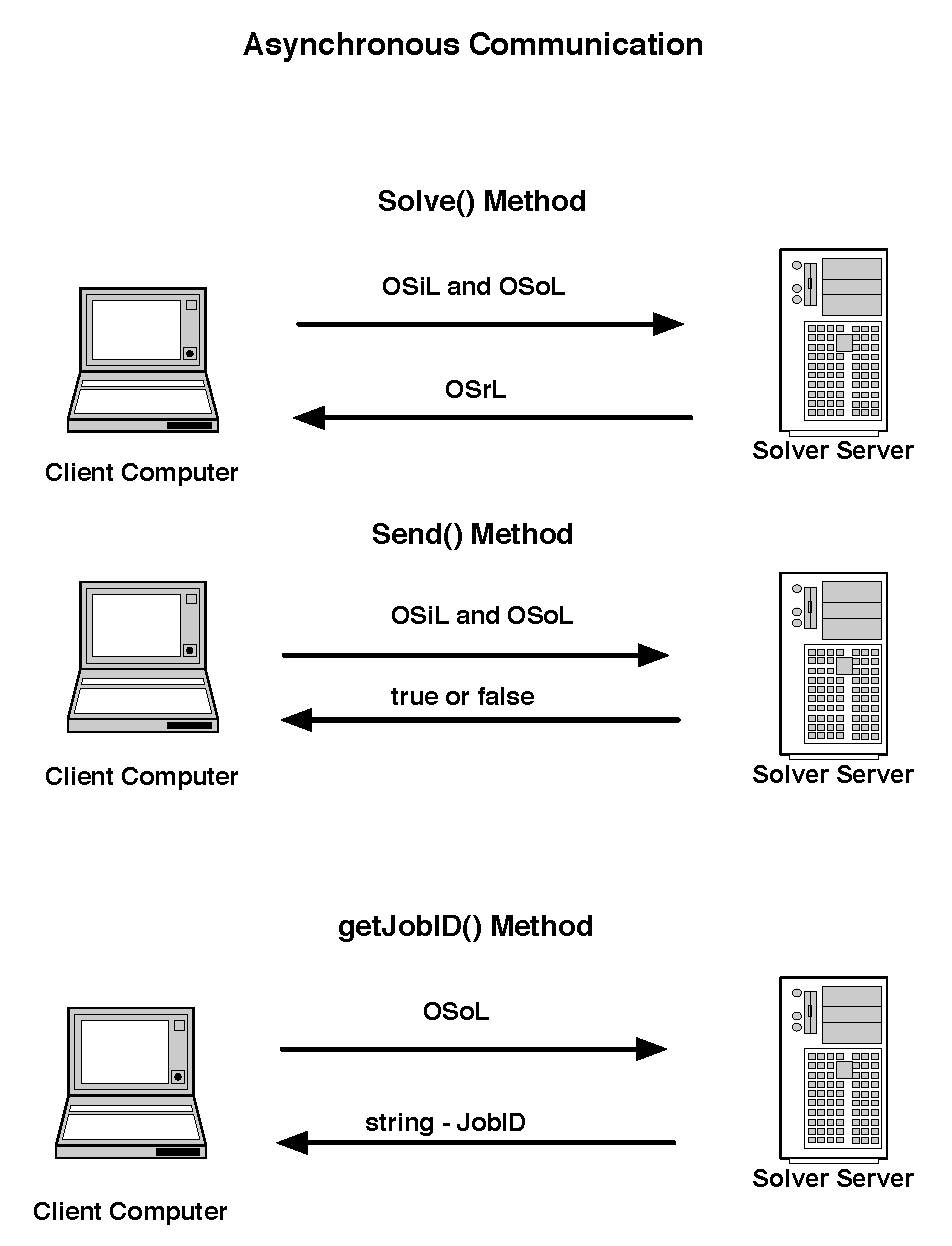
\includegraphics[scale=0.5]{\figurepath/asynchronous1.pdf}
\caption{Input and output for {\tt solve}, {\tt send}, and {\tt getJobID} methods.} 
\label{figure:async1}
\end{figure}


\begin{figure}[ht]
\centering
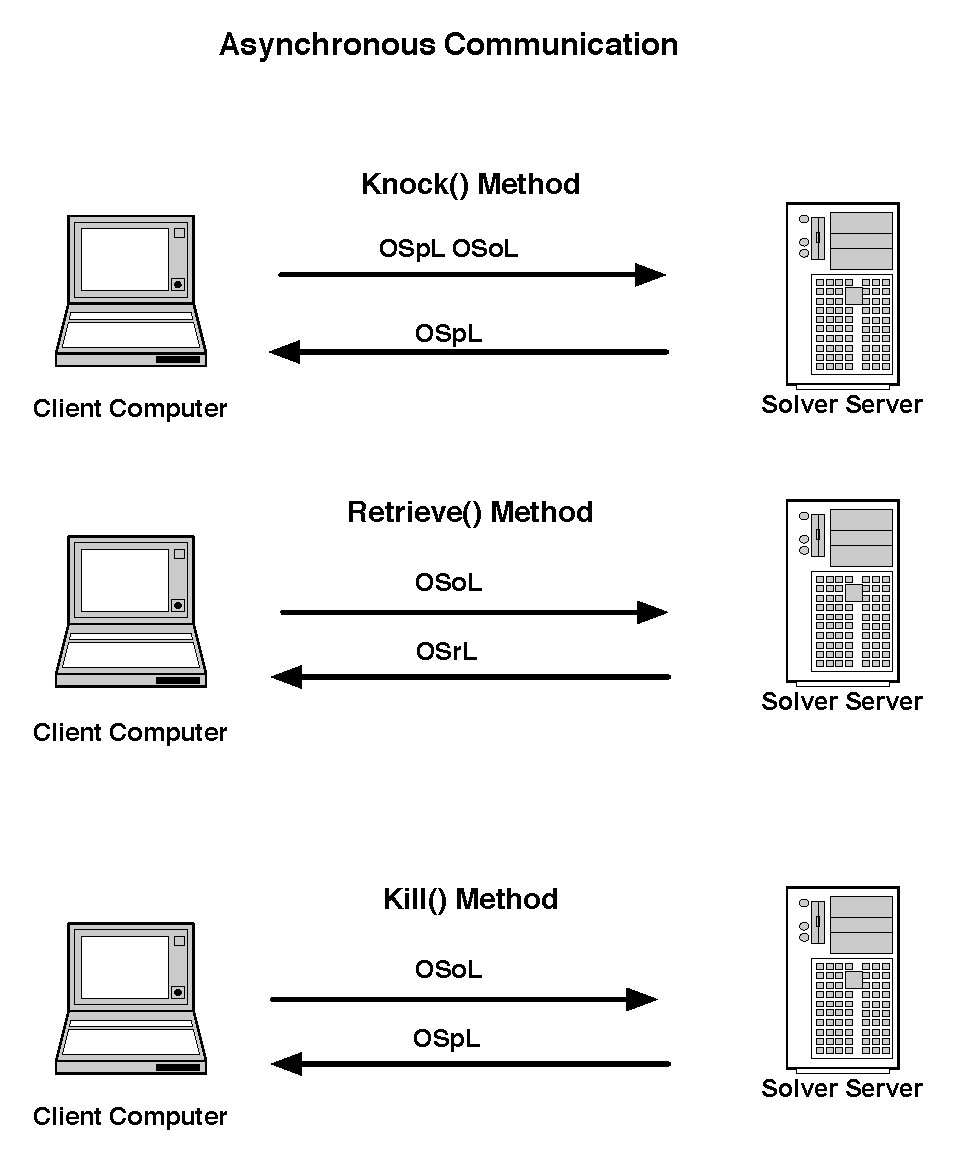
\includegraphics[scale=0.5]{\figurepath/asynchronous2.pdf}
\caption{Input and output for {\tt knock}, {\tt retrieve}, and {\tt kill} methods.} 
\label{figure:async2}
\end{figure}

\section{Setting up a Solver Service with Tomcat}\label{section:tomcat}





\section{Examples}\label{section:examples}

\subsection{AMPL Client:  Hooking AMPL to Solvers}\label{section:amplclient}

The {\tt amplClient} executable is designed to work with the AMPL program. See \url{www.ampl.com}. The {\tt amplClient} acts like an AMPL ``solver.'' The {\tt amplClient} is linked with the OS library and can be used to solve problems either remotely. In both cases the {\tt amplClient} uses the {\tt OSnl2osil} class to convert the AMPL generated nl file (which represents the problem instance) into the corresponding instance representation in the OSiL format.  

For example, assume that there is a problem instance, {\tt hs71.mod} in AMPL model format. To solve this problem locally by calling the {\tt amplClient} from AMPL first start AMPL and then execute the following commands. In this case we are assuming that the local solver used is {\tt Ipopt.} 

\begin{verbatim}
# take in problem 71 in Hock and Schittkowski 
# assume the problem is in the AMPL directory
model hs71.mod;
# tell AMPL that the solve is amplClient
option solver amplClient;
# now tell amplClient to use Ipopt
option amplClient_options "solver ipopt";
# the name of the nl file (this is optional)
write gtestfile;
# now solve the problem
solve;
\end{verbatim}

This will invoke {\tt Ipopt} locally and the result in OSrL format will be displayed on the screen. In order to call a remote solver service, after the command
\begin{verbatim}
option amplClient_options "solver ipopt";
\end{verbatim}
provide an option which has the address of the remote solver service.
\begin{verbatim}
option ipopt_options "http://128.135.130.17:8080/os/OSSolverService.jws";
\end{verbatim}

\subsection{CppAD:  Using the CppAD Algorithmic Differentiation Package}\label{section:cppad}

\subsection{File Upload:  Using a File Upload Package}\label{section:fileupload}

\subsection{Instance Generator: Using the OSInstance API to Generate Instances}\label{subsection:exampleOSInstance}

\section{References}

Kipp -- put in some links to OSiL paper and INFORMS talks.

\section{Appendix}\label{section:appendix}

This is the complete OSiL representation for the optimization problem given in (\ref{eq:roobj})--(\ref{eq:ro3}). 


{\normalsize \baselineskip 16pt \vspace{2pt}
\begin{verbatimtab}[5]
<?xml version="1.0" encoding="UTF-8"?>
<osil xmlns="os.optimizationservices.org">
	<instanceHeader>
		<name>Modified Rosenbrock</name>
		<source>Computing Journal 3:175-184, 1960</source>
		<description>Rosenbrock problem with constraints</description>
	</instanceHeader>
	<instanceData>
		<variables numberOfVariables="2">
			<var lb="0" name="x0" type="C"/>
			<var lb="0" name="x1" type="C"/>
		</variables>
		<objectives numberOfObjectives="1">
			<obj maxOrMin="min" name="minCost" numberOfObjCoef="1">
				<coef idx="1">9.0</coef>
			</obj>
		</objectives>
		<constraints numberOfConstraints="2">
			<con ub="25.0"/>
			<con lb="10.0"/>
		</constraints>
		<linearConstraintCoefficients numberOfValues="3">
			<start>
				<el>0</el><el>2</el><el>3</el>
			</start>
			<rowIdx>
				<el>0</el><el>1</el><el>1</el>
			</rowIdx>
			<value>
				<el>1.</el><el>7.5</el><el>5.25</el>
			</value>
		</linearConstraintCoefficients>
		<quadraticCoefficients numberOfQuadraticTerms="3">
			<qTerm idx="0" idxOne="0" idxTwo="0" coef="10.5"/>
			<qTerm idx="0" idxOne="1" idxTwo="1" coef="11.7"/>
			<qTerm idx="0" idxOne="0" idxTwo="1" coef="3."/>
		</quadraticCoefficients>
\end{verbatimtab}
   \newpage
\begin{verbatimtab}[5]
		<nonlinearExpressions numberOfNonlinearExpressions="2">
			<nl idx="-1">
				<plus>
					<power>
						<minus>
							<number type="real" value="1.0"/>
							<variable coef="1.0" idx="0"/>
						</minus>
						<number type="real" value="2.0"/>
					</power>
					<times>
						<power>
							<minus>
								<variable coef="1.0" idx="0"/>
								<power>
									<variable coef="1.0" idx="1"/>
									<number type="real" value="2.0"/>
								</power>
							</minus>
							<number type="real" value="2.0"/>
						</power>
						<number type="real" value="100"/>
					</times>
				</plus>
			</nl>
			<nl idx="1">
				<ln>
					<times>
						<variable coef="1.0" idx="0"/>
						<variable coef="1.0" idx="1"/>
					</times>
				</ln>
			</nl>
		</nonlinearExpressions>
	</instanceData>
</osil>
\end{verbatimtab}

}% end


\bibliography{\bibpath/kippbib}

\end{document}

